\documentclass[11pt,a4paper,oneside]{report}

\usepackage{url, enumitem}
\usepackage{amsfonts, amsmath}
\usepackage{graphicx, color}
\usepackage{algorithm}
\usepackage[toc,page]{appendix}
\usepackage{lmodern}

% Some useful macros.
\newcommand{\given}{\,|\,}
\newcommand{\R}{\mathbb{R}}
\newcommand{\E}{\mathbb{E}}
\newcommand{\var}{\text{var}}
\newcommand{\cov}{\text{cov}}

\usepackage{float}
\floatplacement{figure}{H} % force figures to be placed always at defined position!
\begin{document}

\title{CS 283: Initial Proposal}
\author{Nicolas Drizard \\
Leonhard Spiegelberg}
\date{10/23/15}

\maketitle

\newpage

\section*{Introduction}

Looking for an applied project, we decided to take part in a Kaggle competition: Right Whale Recognition! The objective of this competition is to build a program to recognize right whales in aerial photographies, given a training set with $500$ (North Atlantic) right whales. The dataset is constituted of $11,468$ aerial photographies with only one whale. Among these pictures, $4,545$ are already labeled with the ID of one of the 500 whales. The main characteristics which help to differentiate one whale from another are the white callosities (roughened patches of skin) on their head.\\
\\

In this proposal, we first discuss some of the challenges of this problem and then present a potential roadmap to address this problem.


\section*{Challenges}

One of the main challenges with this problem relies in the feature engineering part. The images are raw pictures taken by a scientist with a normal camera and the whale is most of the time hard to recognize even with the naked eye. Different elements may perturb our work:
\begin{itemize}
	\item different lighting conditions need to addressed in the preprocessing step
	\item foam on the water has nearly the same color like the callosities we want to recognize. As foam takes nearly every shape, this will cause a lot of 'foam' features that will be incorrectly classified as callosities
	\item the orientation and position of the whale impacts visibility of the features, i.e. the whale can be half or more covered by water. Water refraction will change feature appearance.
\end{itemize}


\section*{Roadmap}
Given the lack of relevant information and the high level of noise in the pictures, we will use a progressive approach to solve this problem. \\
First, we will select a set of nice images (no distraction like foam, visible key features) to work on the feature engineering part to have a better understanding of the problem.\\
On these pictures, we will extract features. Two approaches may be considered. On the first hand, we extract a bag of features for each image (with SIFT for instance) and apply an algorithm to select the relevant features among them, i.e. the whale based one, and compare them (with a POOF approach for instance). On the other hand, we want to select directly the relevant features. Working on nice images makes this task easier as the noise is reduced. Then, we can apply the following classical feature extraction workflow:
\begin{enumerate}
	\item Preprocessing (i.e. normalizing luminance, converting channels, ...)
	\item Thresholding (extract pixels of interest, i.e. via a hysteresis approach)
   	\item Segmentation (Splitting the points into segments)
    	\item Feature estimation for each segment (i.e. half axes of ellipses, roundness measures, ...)
\end{enumerate}
Once we come up with relevant features, we run a classifier on the training set. We will focus on the feature engineering part so we will probably use a classical classifier as for instance SVM or regularized logistic regression. 

\begin{appendices}
\chapter*{Whale Pictures}

\begin{figure}
	\centering
	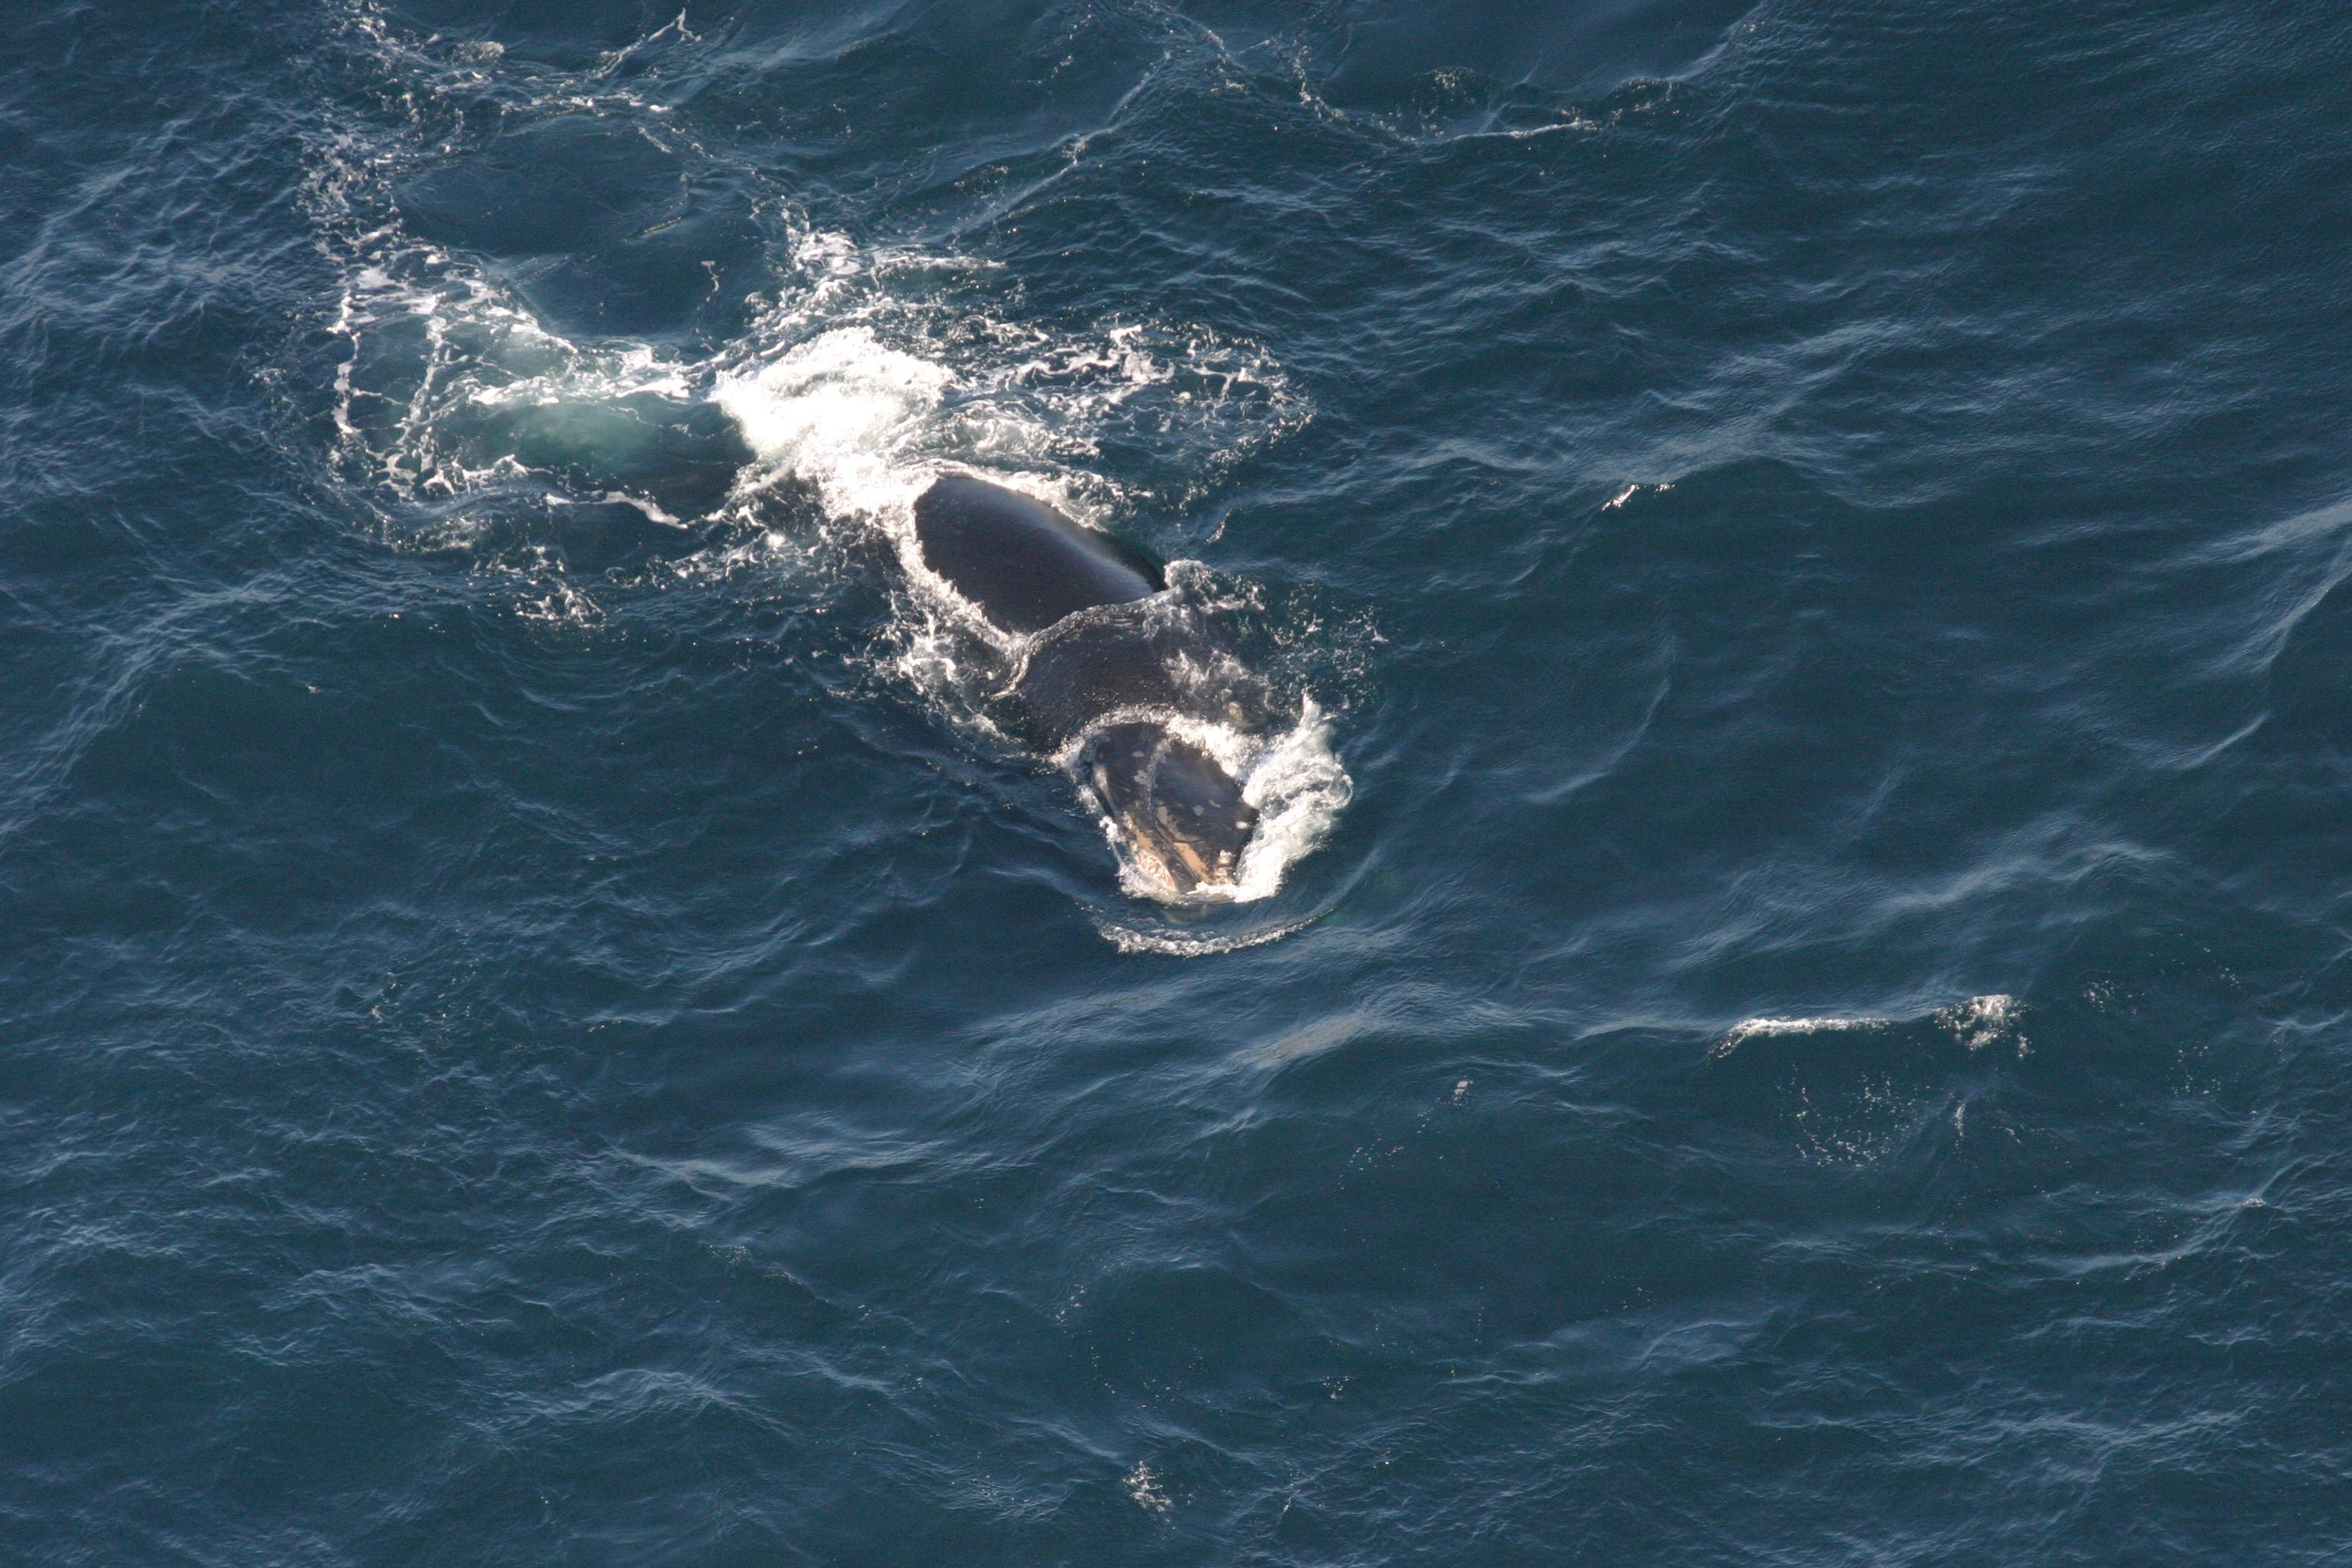
\includegraphics[scale=0.1]{foam.jpg}
	\caption{Example of a whale aerial picture with foam}
\end{figure}

\begin{figure}
	\centering
	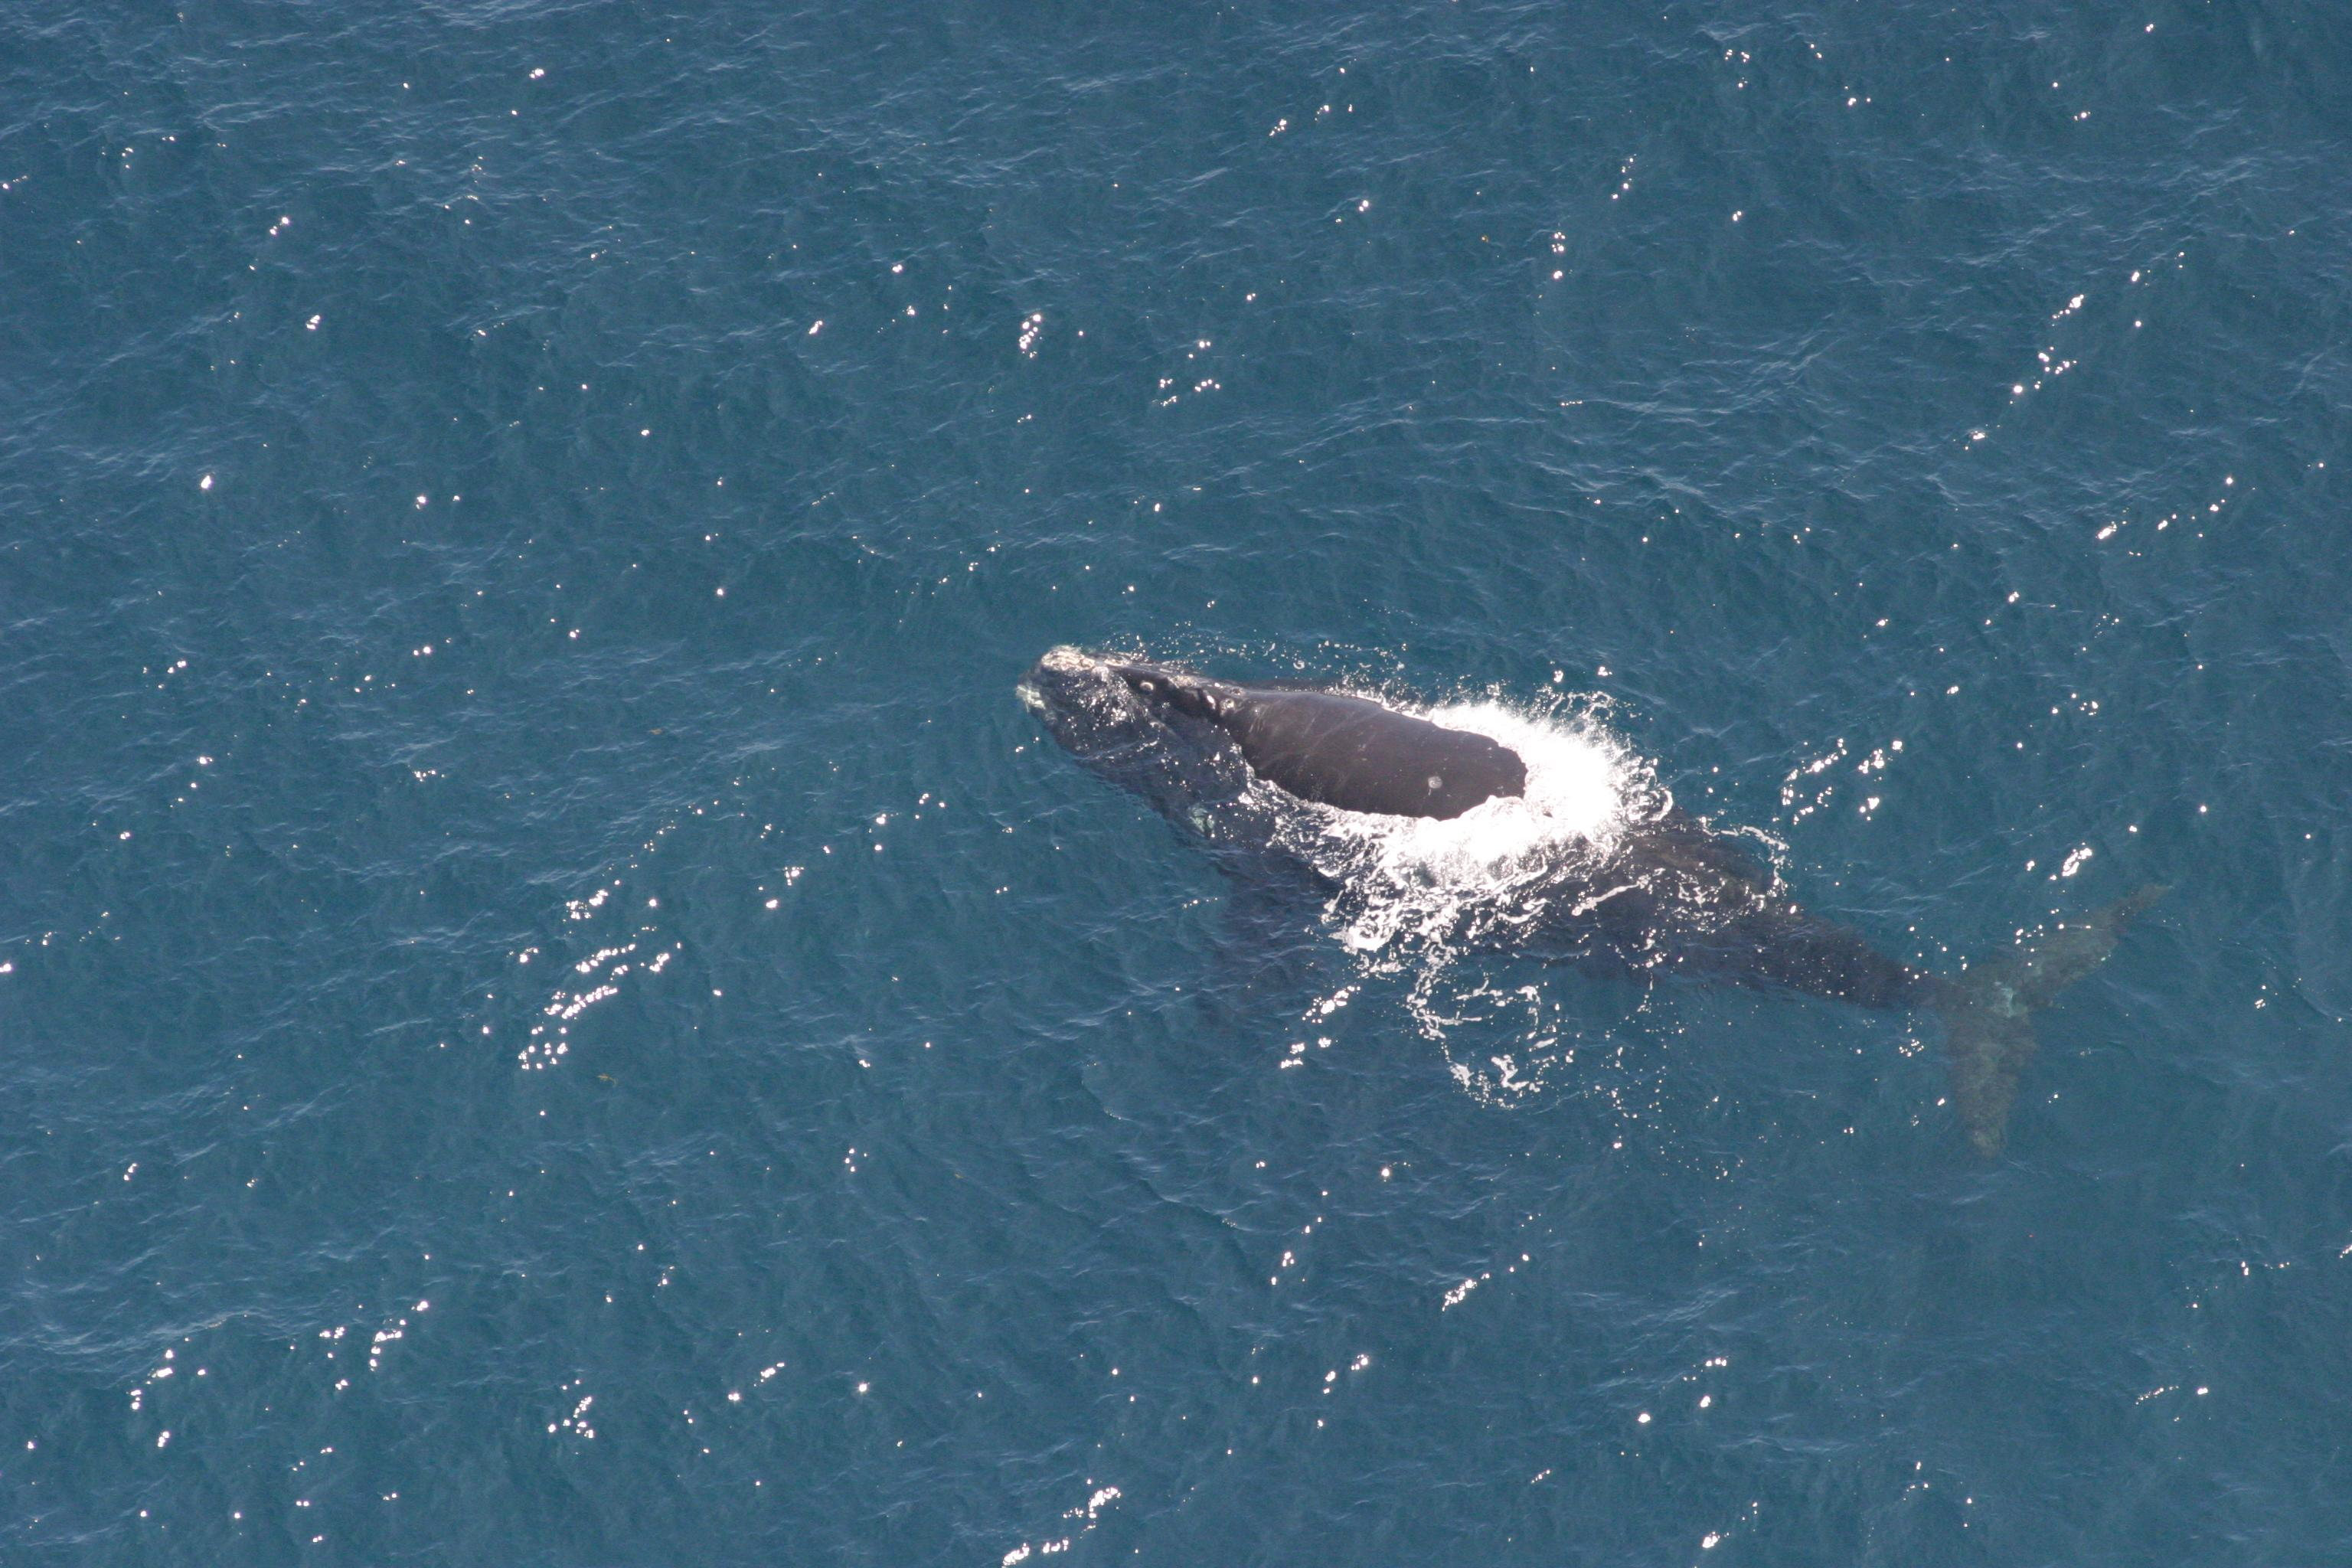
\includegraphics[scale=0.15]{water.jpg}
	\caption{Example of a whale aerial picture with shining water}
\end{figure}

\begin{figure}
	\centering
	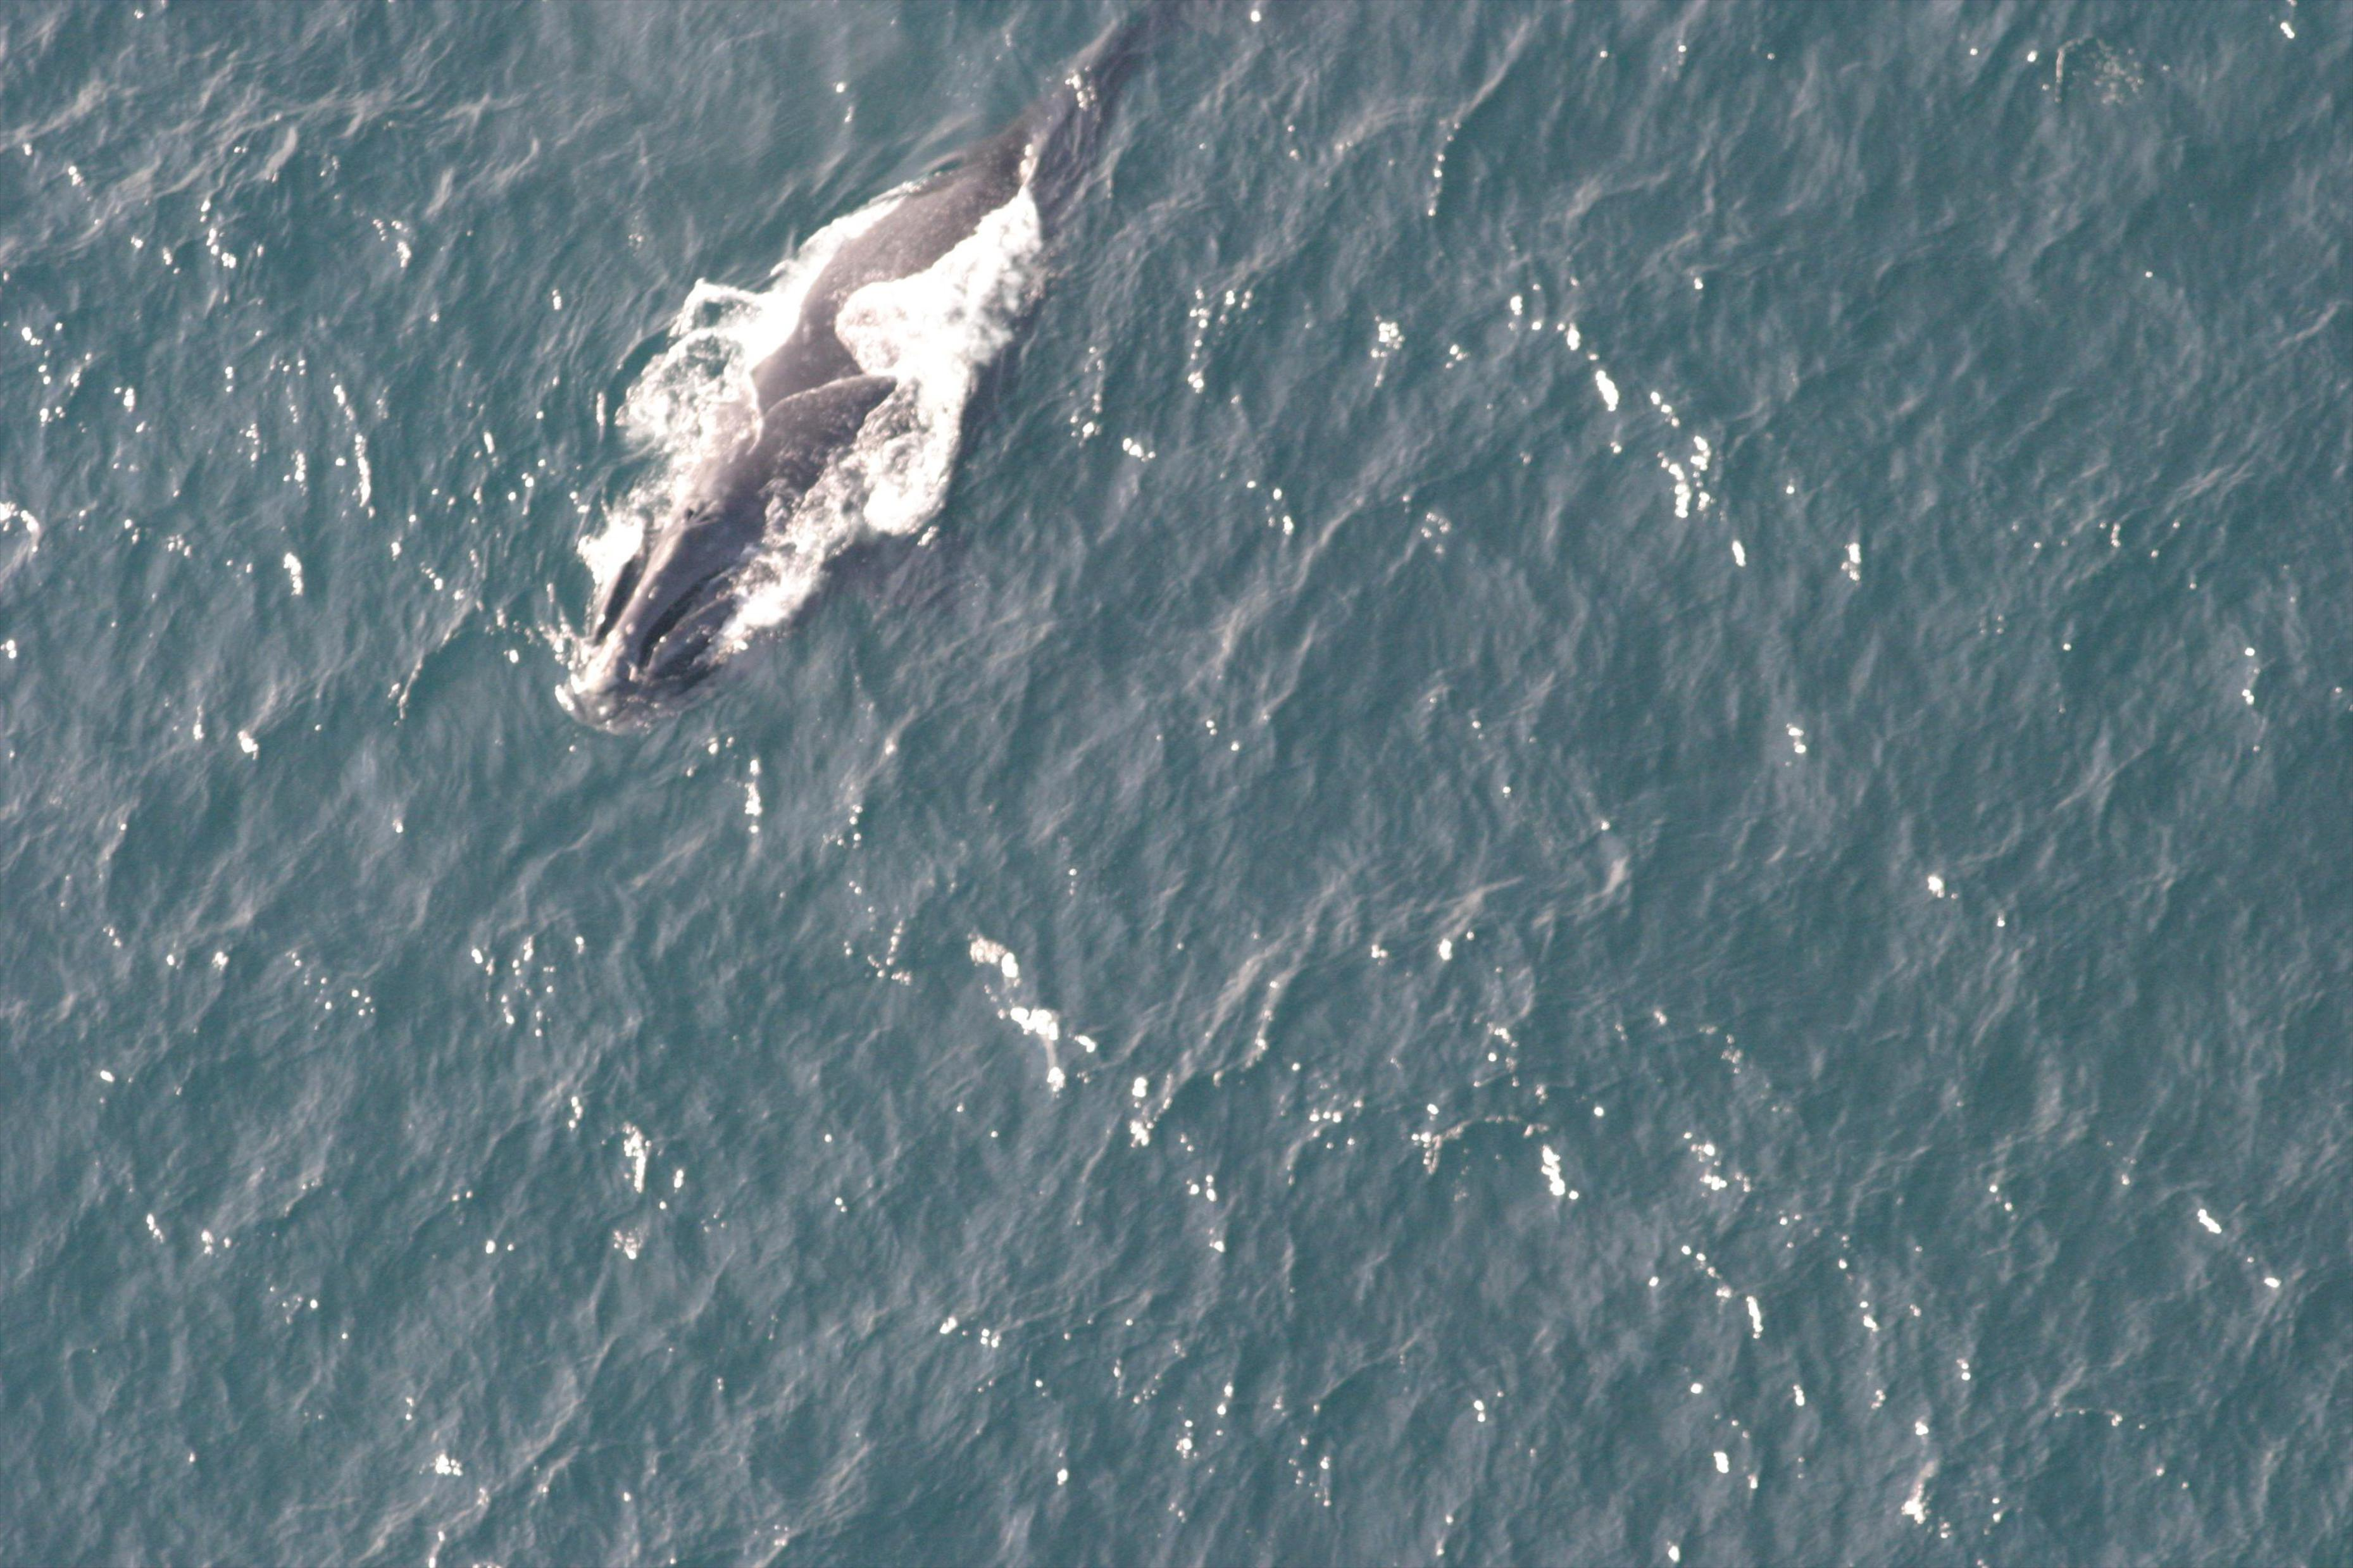
\includegraphics[scale=0.1]{invisible.jpg}
	\caption{Example of a whale aerial picture where the callosities are not visible}
\end{figure}

\begin{figure}
	\centering
	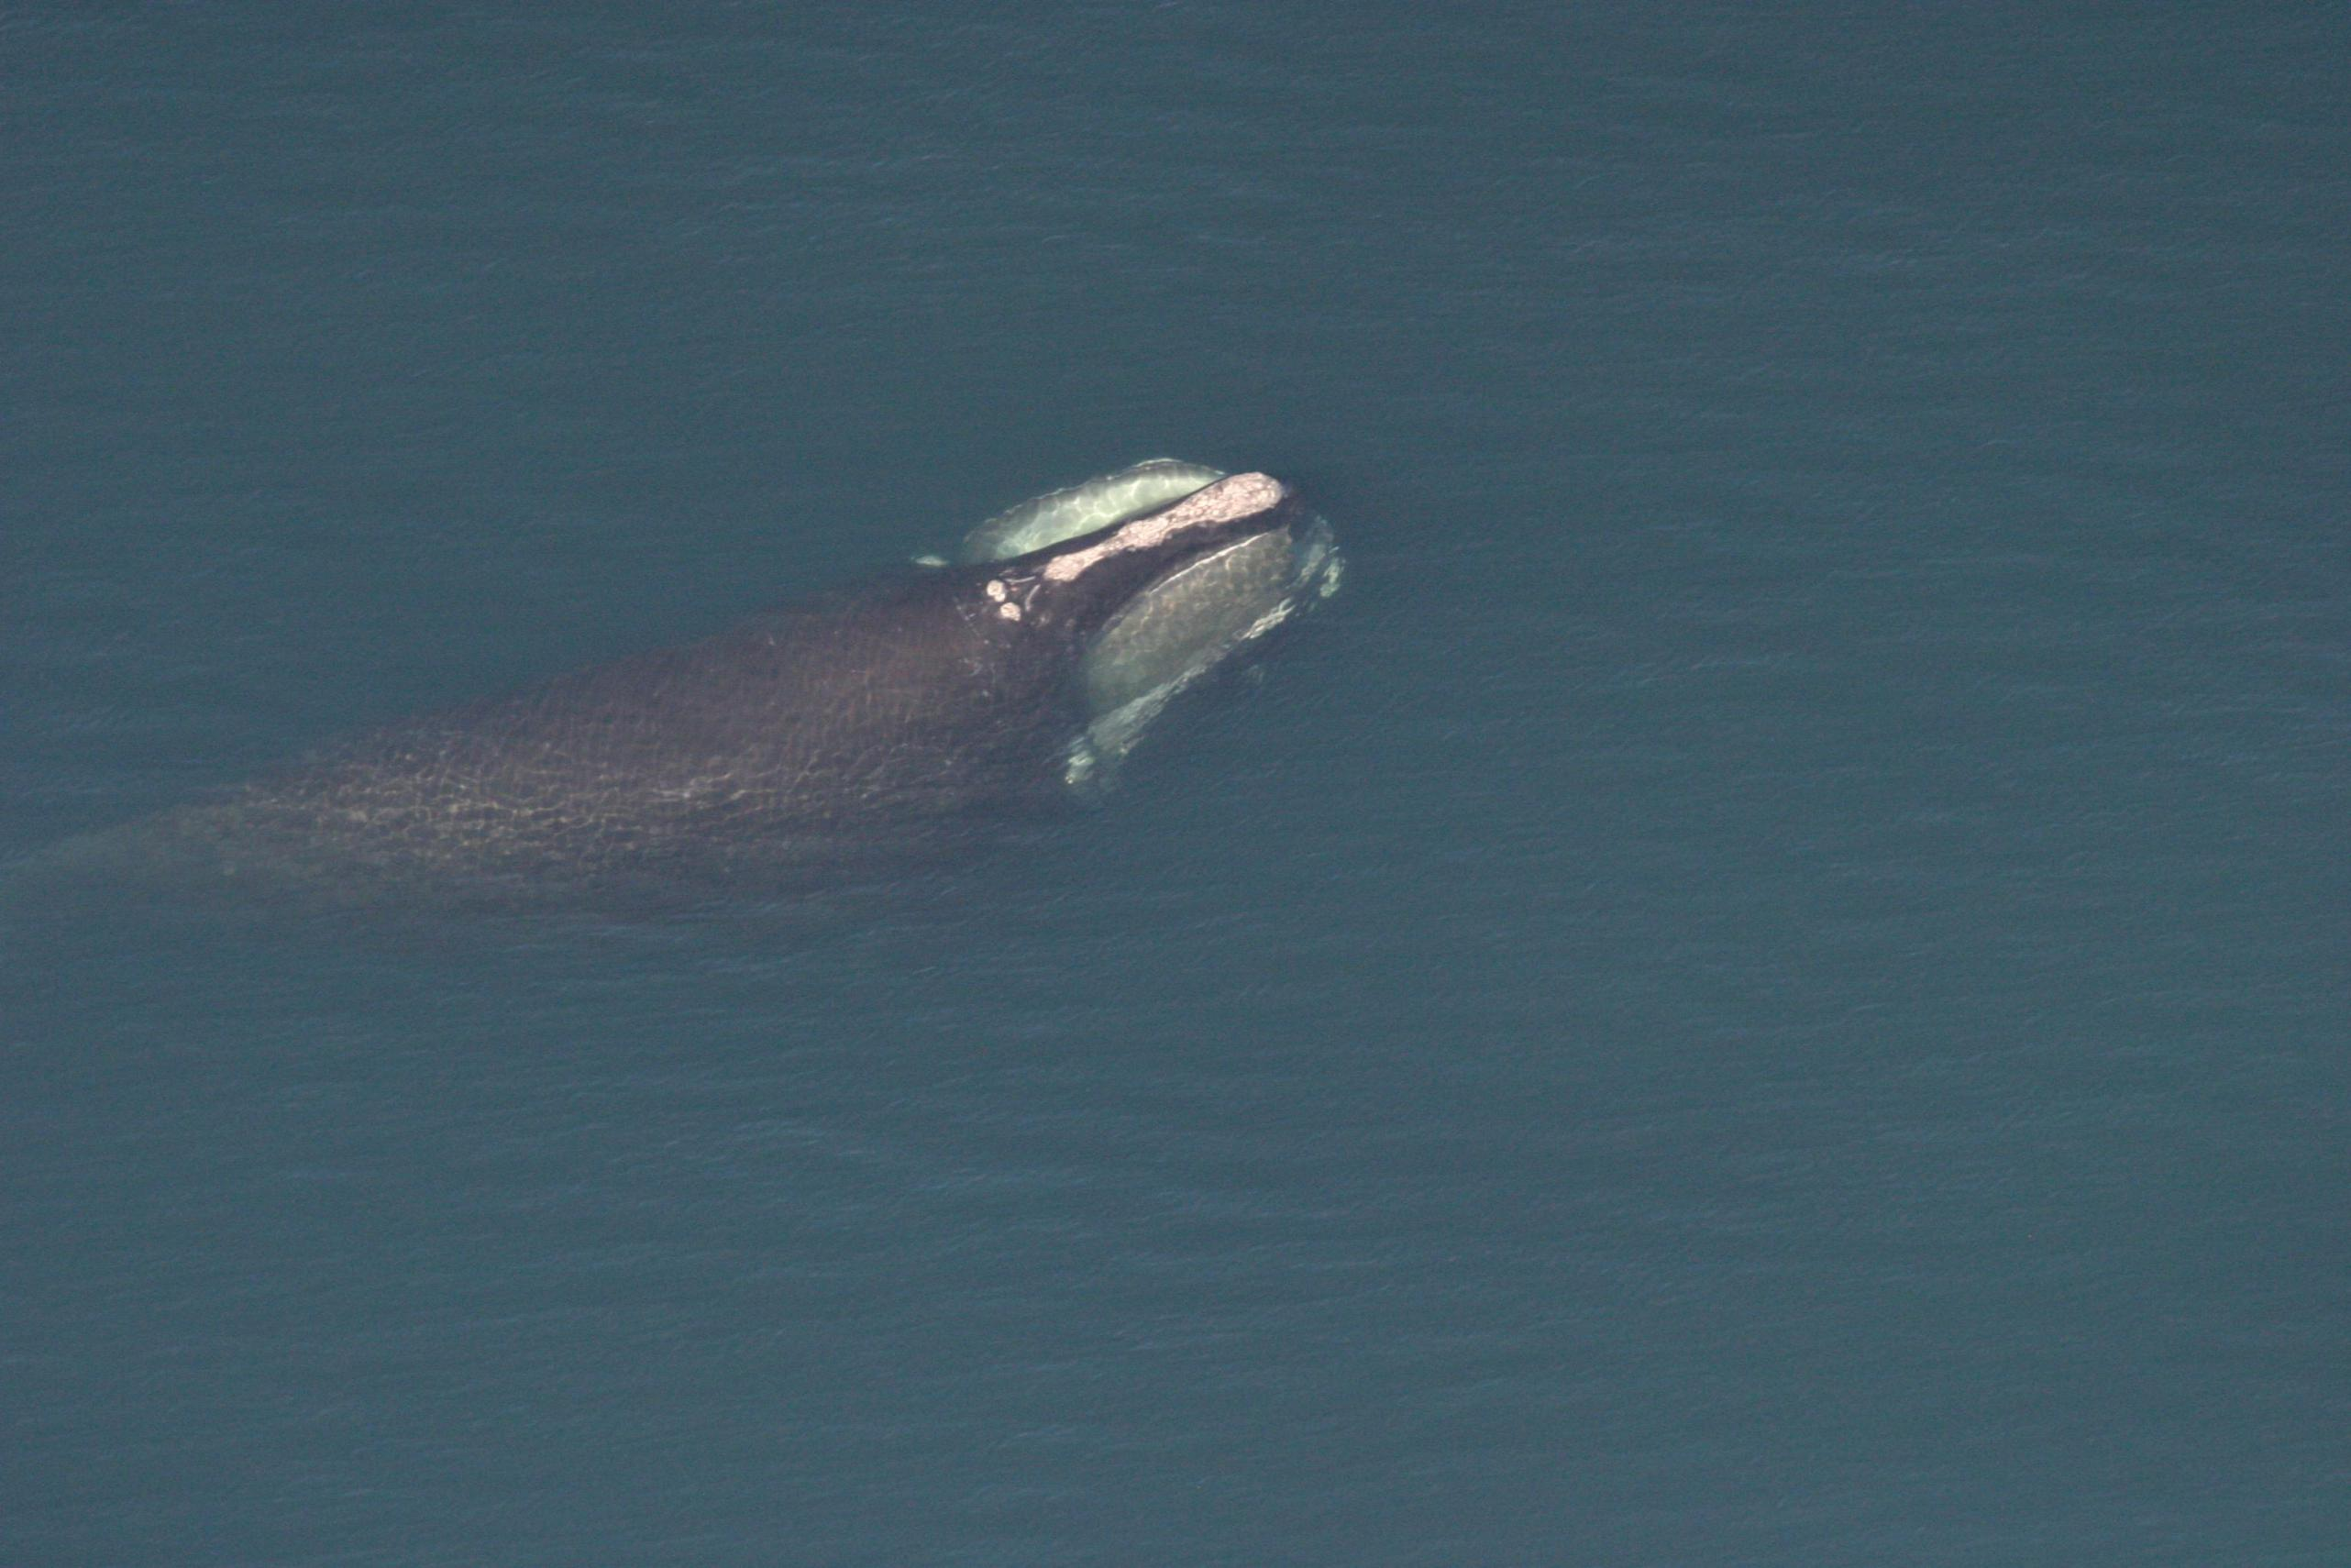
\includegraphics[scale=0.15]{better.jpg}
	\caption{Example of a relevant whale aerial picture}
\end{figure}

\end{appendices}

\end{document}
